\chapter{基于同步内存回收的内存压力量化算法的设计与实现}
\label{chap:基于同步内存回收的内存压力量化算法的设计与实现}
本章详细介绍了基于同步内存回收延迟的内存压力量化算法的设计与实现细节。首先分析了同步回收延迟与内存压力的关联性,然后提出了基于同步回收延迟的内存压力量化算法的设计思想,关键技术细节,最后介绍了该算法的实现细节。

\section{同步内存回收延迟与内存压力的关联性建模}

在内存管理研究中,工作集估计算法作为核心组件,其精确性直接影响内存分配策略与页面置换决策的效能。如\ref{sec:工作集估计算法研究历史与现状}节所述,现有工作集估计方法可归纳为三类典型范式:基于统计采样的近似计算模型、依托系统运行时特征的启发式预测算法,以及基于机器学习模型的离线训练-在线预测框架。然而,机器学习算法在面对新型应用场景时存在泛化能力不足的问题,其预测性能有待进一步验证。

基于统计特征的启发式算法在内存管理领域被广泛应用,原因在于它们能够实时适应系统运行状态的变化,满足动态内存管理的需求。在这类算法中,内存压力指标是一个核心概念,它量化了系统内存资源的紧张程度,为内存卸载决策提供了重要依据。现有研究通常采用缺页中断频率、页面分配速率等多种统计指标来表征内存压力,并通过这些指标来估计工作集大小。然而,这些传统方法存在两个关键缺陷:

\begin{itemize}
    \item 内存压力指标与工作集大小的函数关系呈现显著的非线性特征。例如,工作集转换可能导致大量缺页中断,从而干扰算法对工作集大小的准确判断。
    \item 内存压力指标未充分考虑异构存储设备在性能上的显著差异。以机械硬盘与NVM为例,二者可能发生相同次数的缺页中断,但其处理压力存在显著差异。由于NVM能够快速处理缺页中断,在不影响性能的前提下,可适当缩小工作集以节约内存资源。
\end{itemize}

本研究基于Linux内核同步内存回收机制提出新型压力度量指标,其数学表征为:
\begin{equation}
    \label{eq:mem_pressure}
    mem\_pressure = \frac{T_{sync}}{T_{epoch}}
\end{equation}

其中\(T_{sync}\)表示同步回收累积耗时,\(T_{epoch}\)为监控时间窗口。\(T_{sync}\)可通过在Linux内核的 \_\_alloc\_pages\_direct\_reclaim 函数入口和出口处插桩,记录每次同步回收操作的开始和结束时间戳,并在时间窗口内对所有回收操作的持续时间进行累加得到。\(T_{epoch}\) 表示一个完整的监控时间窗口,通常设置为系统的采样周期,例如2秒。 mem\_pressure 的取值范围为 [0, 1]。当 mem\_pressure 接近0时,表示系统几乎没有内存压力:当其接近1时,表示系统几乎所有时间都在进行同步内存回收,此时系统处于严重的内存压力状态,性能将显著下降。

该内存压力指标的提出基于以下理论分析:

\begin{enumerate}
    \item 当系统内存充足时,同步回收操作极少发生,\(T_{sync}\) 接近于零;
    \item 当内存压力逐渐增加时,\(T_{sync}\) 呈现出与压力程度近似线性的增长;
    \item 对于异构存储后端,高性能设备(如NVM)处理同等数量的缺页中断所需时间更短,计算得到的内存压力值也相应较低,准确反映了实际系统状态。
\end{enumerate}

该方法直接测量因内存压力导致的性能损失时间,而非间接指标。同步内存回收发生时,应用程序必然被阻塞,这部分时间的占比直接反映了应用因内存不足而遭受的性能损失,建立了内存压力与性能影响之间的直接联系。

在异构卸载环境中,该方法能够自动适应不同存储后端的性能特性。对于高性能存储设备(如NVM或Optane),即使发生相同次数的缺页中断,由于其处理速度更快,测得的同步回收时间会相应减少,从而体现出较低的内存压力值;而对于传统机械硬盘,相同次数的缺页中断会导致更长的回收时间,反映出更高的性能损失和内存压力。这种适应性消除了传统方法中需要为不同存储设备单独调整评估参数的复杂性。

无论应用程序是内存密集型、计算密集型还是I/O密集型,当内存不足导致性能下降时,都会表现为同步回收时间的增加。这使得该方法能够在不同类型的工作负载下保持一致的评估标准,无需针对特定应用类型进行定制化调整。

基于上述理论分析,下一节将详细介绍如何设计和实现基于同步内存回收延迟的内存压力量化算法,包括多核系统中的加权聚合策略、指数移动平均平滑处理以及定点数优化技术。

\section{基于同步内存回收延迟的内存压力量化算法}
\label{sec:基于同步内存回收延迟的内存压力量化算法}

在 \ref{sec:Linux内存回收机制} 节中,已经对 Linux 内核同步内存回收机制做了详细的分析,分析表明,函数 \_\_alloc\_pages\_direct\_reclaim 的执行时间是反映同步回收延迟的重要指标。基于此本节提出了一种内存压力检测方法。该方法利用内核插桩技术,在 \_\_alloc\_pages\_direct\_reclaim 函数的入口和出口处改变状态,然后在内核中每次发生同步中断的时候去更新累计时间和CPU的非空闲时间,从而直接获取每次同步回收操作的耗时。为了综合反映多  CPU  系统中不同核心的负载差异,本研究引入了多  CPU  加权聚合策略。此外,为了平滑压力数据、减少短期波动的影响,本研究采用了指数移动平均算法。此外,还采用了定点数优化技术,显著提高了计算效率。

\subsection{多核加权聚合}
\label{sec:weighted_aggregation}
本研究通过插桩技术得到的是各处理器核心在同步内存回收过程中的阻塞时间 \(T_c^{block}\),其中 \(c\) 表示核心编号,需要将多个核心的 \(T_c^{block}\) 聚合为一个压力值。然而,采用简单的算术平均方法计算系统压力:
\begin{equation}
    \label{eq:simple_average_pressure}
    Pressure_{simple} = \frac{\sum_{c=1}^{n} T_c^{block}}{\Delta T \times n} \times 100\%
\end{equation}

其中,\(\Delta T\) 为采样周期,\(n\) 为处理器核心数量,简单平均算法在多核系统中存在两个关键理论缺陷,影响其准确表征系统内存压力的能力。

首先,简单平均算法忽略了处理器核心间负载分布的不均衡性,导致所谓的空闲核心稀释效应(idle core dilution effect)。在异构负载环境中,当少数核心承担主要计算任务而其他核心相对空闲时,高负载核心所反映的内存压力信号会被空闲核心的数据稀释。以四核系统为例,若其中一个高负载核心记录了0.5秒的同步回收阻塞时间,一个轻负载核心记录了0.1秒,而其余两个核心几乎无阻塞(均为0秒),则系统压力计算结果为:
\[
Pressure_{simple} = \frac{0.5 + 0.1 + 0 + 0}{1.0 \times 4} \times 100\% = 15\%
\]

此结果明显低估了系统实际承受的内存压力,因为对于执行关键任务的处理器核心而言,50\%的时间(0.5秒/1.0秒)被阻塞在内存回收操作上,这种严重的资源受限状态在平均计算中被显著弱化。

其次,简单平均算法对所有核心赋予等价权重,未能反映不同核心在系统整体性能中的贡献差异。在工作负载不均衡的场景下,主要完成计算任务的核心对系统性能的影响更为显著。考虑一个双核系统,\(\Delta T\) 为100ms。核心0处于高负载状态,非空闲时间为90ms(占总时间的90\%用于处理任务),其中60ms用于同步内存回收,30ms用于处理其他任务;而核心1基本处于轻负载状态,非空闲时间仅20ms(占总时间的20\%),其中10ms用于同步内存回收,10ms用于处理其他任务。简单平均算法计算得出的系统压力为:
\[
Pressure_{simple} = \frac{60 + 10}{100 \times 2} \times 100\% = 35\%
\]

这一结果未能反映核心0作为主要计算资源的压力状态,从而可能导致资源管理决策的偏差。

为克服上述缺陷,本研究提出采用加权聚合算法,这种启发式方法借鉴了多领域中的贡献度加权思想\citing{Hwang1981MultipleAD}。类似的权重分配策略在计算机体系结构中的不对称多处理器调度\citing{petrucci2012lucky}中得到了广泛应用。该算法的核心思想是:根据每个处理器核心的运行时间分配权重。核心的运行时间越长,表明其在采样周期内处理的任务越多,其上发生的同步内存回收事件对系统整体性能的影响也越显著,其行为也更具有代表性。加权聚合算法的计算公式如下:

\begin{equation}
    \label{eq:weighted_aggregation}
    Pressure_{weighted} = \frac{\sum_{c=1}^{n} (T_c^{block} \times W_c)}{\sum_{c=1}^{n} W_c} \times 100\%
\end{equation}

其中,\(T_c^{block}\) 表示核心 \(c\) 在采样周期 \(\Delta T\) 内的同步内存回收总延迟时间,\(W_c\) 表示核心 \(c\) 的权重,即其在采样周期 \(\Delta T\) 内的非空闲时间,非空闲时间直接反映了该核心的有效工作量。分母中的 \(\sum_{c=1}^{n} W_c\) 表示所有核心的非空闲时间总和。通过这种加权方式,算法能够有效降低或消除空闲核心的噪声影响,同时更准确地反映不同核心负载对系统整体性能压力的贡献,从而提供更可靠、更具代表性的内存压力评估结果。应用加权算法于前述双核系统示例,其结果为:
\[
Pressure_{weighted} = \frac{60 \times 90 + 10 \times 20}{90 + 20} \times 100\% = 51\%
\]

表\ref{tab:weighted_vs_simple}直观展示了简单平均与加权聚合算法在三种典型负载场景下的表现差异。可以看出,随着核心负载分布不均衡程度的增加,两种算法计算结果的差异也越显著,尤其在高度不均场景下,简单平均算法严重低估了系统实际内存压力。

\begin{table}[htbp]
    \centering
    \caption{简单平均与加权聚合算法在不同核心负载条件下的比较}
    \label{tab:weighted_vs_simple}
    \begin{tabular}{lccc}
        \toprule
        \multirow{2}{*}{\textbf{负载场景}} & \multicolumn{2}{c}{\textbf{每核心数据}} & \multirow{2}{*}{\textbf{系统压力计算结果}} \\
        \cmidrule(lr){2-3}
         & \textbf{阻塞时间 $T_c^{block}$ (ms)} & \textbf{非空闲时间 $W_c$ (ms)} & \\
        \midrule
        \multirow{4}{*}{均匀负载} & 核心0: 400 & 核心0: 800 & 简单平均: 50\% \\
         & 核心1: 400 & 核心1: 800 & 加权聚合: 50\% \\
         & 核心2: 400 & 核心2: 800 & (两种方法结果相同) \\
         & 核心3: 400 & 核心3: 800 & \\
        \midrule
        \multirow{4}{*}{中度不均} & 核心0: 600 & 核心0: 900 & 简单平均: 40\% \\
         & 核心1: 400 & 核心1: 700 & 加权聚合: 47\% \\
         & 核心2: 300 & 核心2: 500 & (加权方法更准确) \\
         & 核心3: 100 & 核心3: 100 & \\
        \midrule
        \multirow{4}{*}{高度不均} & 核心0: 800 & 核心0: 950 & 简单平均: 27.5\% \\
         & 核心1: 300 & 核心1: 500 & 加权聚合: 63\% \\
         & 核心2: 0 & 核心2: 50 & (简单平均严重低估) \\
         & 核心3: 0 & 核心3: 0 & \\
        \bottomrule
    \end{tabular}
\end{table}


\subsection{指数移动平均算法}
\label{sec:exponential_smoothing}
在获取基于处理器核心的非空闲时间加权的内存压力指标后,本研究进一步考虑压力数据的平滑性以及长期趋势的分析。原始的压力数据(无论是简单平均还是加权平均)可能会因为短暂的、偶然的事件而产生剧烈波动,这些波动可能会掩盖真实的压力趋势。因此,需要采用一种有效的方法对压力数据进行平滑处理,以减少短期波动的影响,同时保留长期趋势信息。指数移动平均(Exponential Moving Average, EMA)算法\citing{gardner1985exponential}在多个方面优于传统平滑方法:首先,相较于简单移动平均(SMA),EMA能更快地响应压力变化;其次,与加权移动平均(WMA)相比,EMA的计算效率更高且内存占用更小;最后,相比于Kalman滤波等复杂算法,EMA具有参数调整简单、计算开销低等优势,特别适合资源受限的实时操作系统环境。

EMA 算法的核心思想是对新旧数据进行加权平均,但与简单算术平均赋予所有数据相同权重不同,EMA 赋予旧数据的影响随时间推移呈指数衰减。这种处理方式更符合实际系统的运行特征:最近发生的事件对当前系统状态的影响通常更大,而较早发生的事件的影响则逐渐减弱。具体来说,EMA 的计算公式为:
\begin{equation}
    EMA_{new} = EMA_{old} \times \alpha + P_{current} \times (1 - \alpha)
    \label{eq:EMA}
\end{equation}

其中,\(EMA_{new}\) 和 \(EMA_{old}\) 分别代表当前时刻和上一时刻的 EMA 值,\(P_{current}\) 是当前时刻的压力值,\(\alpha\) 是一个介于 0 和 1 之间的衰减因子(也称平滑因子)。衰减因子 \(\alpha\) 的数值范围具有明确的物理意义:当 \(\alpha\) 接近 1 时,系统对历史数据的依赖性较高,对新数据的敏感度较低,产生的平滑曲线更加稳定但响应滞后;当 \(\alpha\) 接近 0 时,系统对当前数据的重视度高,对历史数据影响较小,平滑曲线能够快速响应压力变化但可能保留更多短期波动。衰减因子 \(\alpha\) 决定了旧数据影响力衰减的速度,也即决定了 EMA 对历史数据的记忆长度。为了便于参数设置,本文将 \(\alpha\) 与系统可观测参数关联,定义计算关系式为:
\begin{equation}
\alpha = e^{-\Delta T / \tau}
\label{eq:alpha}
\end{equation}

其中,\(\Delta T\) 是采集内存压力数据的周期(例如,每2秒采样一次),\(\tau\) 则反映了希望EMA追踪的压力趋势的时间尺度(例如,10秒、60秒或300秒)。根据公式(\ref{eq:alpha}),当 \(\tau\) 越大时,\(\alpha\) 越接近1,EMA曲线越平滑,对短期波动的抑制能力越强,但对真实压力变化的反应也越迟钝;反之,当 \(\tau\) 越小时,\(\alpha\) 越接近0,EMA曲线对新数据的响应越灵敏,但平滑效果也越差。

相比于简单平均或固定窗口的移动平均算法,EMA 算法具有显著优势。首先,EMA 算法的计算非常高效。它仅需存储上一时刻的 EMA 值,无需维护一个包含大量历史数据的窗口,计算复杂度为 \(O(1)\)。这使得 EMA 非常适合于资源受限的嵌入式系统或需要高频采样的实时监控系统。其次,EMA 算法的参数可调性提供了极大的灵活性。通过调整衰减因子(即调整时间窗口),可以在快速响应和数据平滑之间找到最佳平衡点。这使得 EMA 能够适应不同的应用场景和性能需求。最后,也是最重要的一点,EMA 算法能够有效地追踪压力数据的长期趋势。它不仅能平滑短期波动,还能清晰地展现压力随时间变化的整体走向,帮助及时发现潜在的性能瓶颈或系统异常。

在整个内存压力监控框架中,EMA算法作为时间维度的数据处理层,接收来自多核加权聚合处理后的压力数据,进一步消除时间维度的噪声干扰,为系统提供稳定的内存压力趋势信息,最终用于指导内存管理决策。

\subsection{时间校准与数据处理优化机制}
\label{sec:time_calibration_and_data_processing}
在高并发环境中,内存压力的精确测量面临调度延迟和数据积压等挑战,可能导致采样周期偏移和统计指标失真。本节从时间校准和数据处理两个维度展开分析,提出了相应的优化机制,确保内存压力量化的准确性和稳定性。

\subsubsection{周期性任务的时间校准}

设理想的任务执行时间序列为等间隔离散点:
\[
t_0, \quad t_0 + T, \quad t_0 + 2T, \quad t_0 + 3T, \quad \dots
\]
其中\(T\)为系统设定的基准周期。然而,受系统负载和调度策略影响,实际执行时刻常呈现非线性偏移:
\[
t_0, \quad t_0 + T + \Delta_1, \quad t_0 + 2T + \sum_{i=1}^2\Delta_i, \quad \dots
\]
其中\(\Delta_i \in \mathbb{R}^+\)表示第\(i\)周期的累积延迟。

这种时间偏移若不加处理,会导致采样间隔不均,影响内存压力的准确评估。为解决此问题,本研究设计了基于相位同步的时间校准算法。该算法通过定义两个关键参数实现:
\begin{align}
    \text{missed\_periods} &= \left\lfloor \frac{\text{now} - \text{expires}}{T} \right\rfloor
    \label{eq:missed_periods} \\
    \text{next\_execution} &= \text{expires} + (\text{missed\_periods} + 1) \times T
    \label{eq:next_execution}
\end{align}

式中,\(\text{now}\)表示当前系统时间戳,\(\text{expires}\)表示上次任务完成时刻。算法首先通过公式\ref{eq:missed_periods}计算当前已错过的完整周期数,然后利用公式\ref{eq:next_execution}确定下次执行时刻,将其映射至最近的理想时间点。这种方法不仅修正了当前周期的偏移,更重要的是通过全局时间重映射,有效抑制了时序偏移的级联传播,确保长期运行时的稳定性。

\subsubsection{积压数据的处理机制}

在内存压力监测过程中,生产者(同步回收监测)和消费者(压力计算)之间的速率不匹配可能导致数据积压,进而引发统计指标异常。针对这一问题,本研究提出了两种互补的处理机制:

\paragraph{截断补偿机制} \quad 在无锁采样环境下,时间记录机制存在固有的竞态条件,可能导致某一周期内记录的时间增量溢出至下一周期。特别是在系统承受持续高压力时,单个周期内累积的时间样本可能超过周期本身的长度,产生超过100\%的非物理压力值。

设当前采样周期长度为\(\textit{period}\),对于任一周期内检测到的累积同步回收时间\(v\),当\(v > \textit{period}\)时,系统执行如下处理:
\begin{equation}
v_{\text{current}} = \min(v, \textit{period}), \quad v_{\text{carryover}} = v - v_{\text{current}}
\end{equation}
其中,\(v_{\text{current}}\)表示当前周期内实际统计的有效累积时间,\(v_{\text{carryover}}\)表示超出阈值的剩余时间,将被递延至下一统计周期处理。

该机制基于以下理论保证:
\begin{enumerate}
    \item 总量守恒原理:截断补偿确保所有记录的时间增量都被计入统计,满足任意连续\(n\)个周期的累积等式:
    \begin{equation}
        \sum_{k=1}^n v_{\text{current}}^{(k)} \equiv \sum_{k=1}^n v^{(k)}
    \end{equation}
    \item 误差非累积性:当时间增量从周期\(P\)溢出至周期\(P+1\)时,根据时间守恒原理,它必然在周期\(P\)中释放了等量的时间,使得误差不会随时间累积。
    \item 时间序列同态性:该机制对原始压力曲线进行了时间保持型变换,延迟报告但不改变曲线的积分特性,确保长期评估的准确性。
\end{enumerate}

\paragraph{指数加速收敛} \quad 当系统连续多个周期未能进行数据更新时,标准的指数移动平均(EMA)算法需要进行适应性调整。回顾公式\ref{eq:EMA}中的标准EMA更新公式:
\begin{equation}
    \text{EMA}_{new} = \alpha \cdot \text{EMA}_{old} + (1-\alpha) \cdot \text{Sample}_{current}
\end{equation}

当系统连续\(n\)个周期未更新时,需要从时刻\(t\)直接推进至时刻\(t+n\)。通过数学归纳法,可以推导此情况下的一般形式:

\begin{equation}
\text{EMA}(t+n) = \alpha^n \cdot \text{EMA}(t) + \sum_{k=1}^{n} \alpha^{n-k} \cdot (1-\alpha) \cdot \text{Sample}(t+k)
\end{equation}

在实际情境中,若连续\(n-1\)个周期无数据更新,仅在第\(n\)个周期获得新样本\(\text{Sample}(t+n)\),则中间缺失的样本值可视为零,上式简化为:
\begin{equation}
\label{eq:EMA_2}
\text{EMA}(t+n) = \alpha^n \cdot \text{EMA}(t) + (1-\alpha) \cdot \text{Sample}(t+n)
\end{equation}

式(\ref{eq:EMA_2})中的\(\alpha^n\)项在\(n\)较大时计算开销显著。为提高效率,本文采用二进制快速幂算法实现:

\begin{algorithm}[htbp]
    \caption{Binary Exponentiation for EMA Acceleration}
    \label{alg:fast_exp}
    \SetAlgoLined
    
    \KwIn{\(x\): base value (real or integer), \(n\): exponent (non-negative integer)}
    \KwOut{\(x^n\): computed power}
    
    result \(\gets 1\)\;
    \While{$n > 0$}{
        \If{$n \,\mathrm{AND}\, 1 \neq 0$}{  \tcp*{Check if lowest bit is 1}
            result \(\gets\) result \(\times\) x\;  \tcp*{Multiply result by current power of x}
        }
        x \(\gets x \times x\)\;  \tcp*{Square x for next iteration}
        n \(\gets n \gg 1\)\;  \tcp*{Right shift n (equivalent to $\lfloor n/2 \rfloor$)}
    }
    \Return result\;
\end{algorithm}

该算法通过将幂运算分解为平方运算和选择性乘法,利用指数的二进制表示实现计算优化。对于任意非负整数\(n\)的二进制表示:
\begin{equation}
n = (b_k b_{k-1} \ldots b_1 b_0)_2 = \sum_{i=0}^{k} b_i 2^i
\end{equation}

幂运算可重写为:
\begin{equation}
x^n = x^{\sum_{i=0}^{k} b_i 2^i} = \prod_{i=0}^k (x^{2^i})^{b_i}
\end{equation}

算法仅需检查\(n\)的每个二进制位,并选择性地将对应\(x\)的幂次项纳入结果,时间复杂度从\(O(n)\)降至\(O(\log n)\),显著提升了系统在处理长期无更新场景时的计算效率。

通过时间校准和数据处理优化机制的协同作用,系统能够在复杂多变的运行环境中保持对内存压力的准确监测,为内存管理决策提供可靠依据。


\subsection{定点数优化}
\label{sec:fixed_point_optimization}

在实时内存压力监测系统中,频繁的数值计算需求对运算效率提出了严格约束。针对内存压力指标计算与 EMA 平滑处理中大量浮点运算可能造成的性能瓶颈,本研究采用基于定点数表示法的优化策略。

\subsubsection{定点数表示原理}

定点数区别于浮点数的动态指数位结构,它通过固定缩放因子将实数映射为整数,从而以移位和整数乘法等高效操作取代复杂的浮点运算。在本系统中,本文定义量化误差为将实数转换为定点数再还原过程中产生的数值偏差。

经过系统分析和性能测试,本研究选取缩放因子$F=2^{10}$,实现Q0.10定点数格式。该选择基于以下考量:$2^{10}=1024$接近$10^3$,便于在十进制系统中理解;同时该精度在内存压力百分比表示(0\%-100\%)场景下能提供约0.1\%的分辨率,满足实时监控需求;此外,$2^{10}$作为2的整数幂,可通过位移操作高效实现乘除运算。

定点数转换过程定义为:将实数$R$通过线性变换映射为整数$D$:
\begin{equation}
D = \lfloor R \cdot F \rfloor
\end{equation}

相应地,定点数还原为实数的计算为:
\begin{equation}
R' = \frac{D}{F}
\end{equation}

\subsubsection{误差分析}

定点数表示不可避免地引入量化误差。定义量化误差$\epsilon$为原始实数$R$与还原实数$R'$之间的差值:
\begin{equation}
\epsilon = R - R' = R - \frac{D}{F} = R - \frac{\lfloor R \cdot F \rfloor}{F} = \frac{\delta}{F} \quad (0 \leq \delta < 1)
\end{equation}

由上式可得,单次量化的绝对误差上界为$\frac{1}{F} = 2^{-10} \approx 0.000977$。对于数值$R \geq 1$的场景,相对误差上界为$\frac{2^{-10}}{R} \leq 0.000977$,即相对误差被限定在千分之一以内,满足内存压力监测的精度要求。

为全面评估定点数在实际计算过程中的误差传播特性,本节分析加减法和乘法两类基本运算的累积误差。

\paragraph{加减法误差分析}\quad 
令实数$R_1$和$R_2$分别被量化为定点数$D_1$和$D_2$,根据量化误差定义,有:
\begin{equation}
|R_1 - \frac{D_1}{F}| \leq \frac{1}{F} \quad \text{和} \quad |R_2 - \frac{D_2}{F}| \leq \frac{1}{F}
\end{equation}

当执行加减法运算时,误差传播遵循:
\begin{equation}
\begin{aligned}
|(R_1 \pm R_2) - \frac{D_1 \pm D_2}{F}| &= |(R_1 - \frac{D_1}{F}) \pm (R_2 - \frac{D_2}{F})| \\
&\leq |R_1 - \frac{D_1}{F}| + |R_2 - \frac{D_2}{F}| \\
&\leq \frac{1}{F} + \frac{1}{F} = \frac{2}{F}
\end{aligned}
\end{equation}

如果将加减法结果再次量化为定点数,可能引入额外的舍入误差,最多为$\frac{1}{F}$。因此,一次加减法操作后再量化的总误差上界为$\frac{3}{F} = 3 \times 2^{-10} \approx 0.002930$,仍然保持在可接受的精度范围内。

在实际实现中,本文采用了误差优化策略:多次连续加减运算只在最终结果上执行一次量化,而非每步操作后都进行量化。这种策略显著减少了中间结果的反复舍入,将$n$次操作的累积误差从最坏情况的$\frac{2n+1}{F}$降低至$\frac{n+1}{F}$。

\paragraph{乘法误差分析}\quad
对于乘法运算,设实数$R_1$和$R_2$分别映射为定点数$D_1$和$D_2$。定点数乘法计算过程为:
\begin{equation}
D_1 \times D_2 = (R_1 \cdot F) \times (R_2 \cdot F) = (R_1 \times R_2) \cdot F^2
\end{equation}

由于结果需要保持Q0.10格式,还需执行右移操作:
\begin{equation}
(D_1 \times D_2) \gg 10 = \lfloor \frac{D_1 \times D_2}{F} \rfloor = \lfloor (R_1 \times R_2) \cdot F \rfloor
\end{equation}

乘法运算中的总误差$\epsilon_{mul}$来源于两部分:
\begin{enumerate}
    \item 输入量化误差:$R_1$和$R_2$量化为$D_1$和$D_2$时各自引入的误差
    \item 结果量化误差:乘法结果右移时的舍入误差
\end{enumerate}

详细分析这两部分误差的传播:

输入量化误差分析:设$R_1 = \frac{D_1}{F} + \epsilon_1$和$R_2 = \frac{D_2}{F} + \epsilon_2$,其中$|\epsilon_1|, |\epsilon_2| \leq \frac{1}{F}$。则:
\[
\begin{aligned}
R_1 \times R_2 &= (\frac{D_1}{F} + \epsilon_1)(\frac{D_2}{F} + \epsilon_2) \\
&= \frac{D_1 \times D_2}{F^2} + \frac{D_1 \times \epsilon_2}{F} + \frac{D_2 \times \epsilon_1}{F} + \epsilon_1 \times \epsilon_2
\end{aligned}
\]

考虑到内存压力监测场景中,$R_1$和$R_2$通常为[0,1]范围内的百分比值或[0,100]范围内的指数衰减因子,可设$|D_1|, |D_2| \leq 100F$。则输入误差传播的上界为:
\begin{equation}
|\frac{D_1 \times \epsilon_2}{F} + \frac{D_2 \times \epsilon_1}{F} + \epsilon_1 \times \epsilon_2| \leq \frac{100}{F} + \frac{100}{F} + \frac{1}{F^2} \approx \frac{200}{F}
\end{equation}

结果量化误差分析:乘法结果右移时的舍入误差上界为$\frac{1}{F}$。

综合两部分误差,定点数乘法运算的总误差上界为:
\begin{equation}
|\epsilon_{mul}| \leq \frac{200}{F} + \frac{1}{F} = \frac{201}{F} \approx \frac{201}{2^{10}} \approx 0.196    
\end{equation}

这一误差上界在极端情况下可能接近0.2,但在实际应用中,典型的内存压力计算场景涉及较小范围的乘数(如\(\alpha \in [0.5, 0.999]\)),实际误差通常维持在\(2^{-9}\)(约0.002)量级,满足系统对精度的要求。

\section{基于同步回收延迟的内存压力量化实现}
\label{sec:基于同步回收延迟的内存压力量化实现}

本节详细阐述前文提出的基于同步回收延迟的内存压力量化算法在Linux内核中的具体实现方案。实现过程面临多核环境下的数据一致性、低开销监测和实时性三大技术挑战,为此本研究设计了基于生产者消费者模式的系统架构。

该实现架构由三个关键组件构成:负责数据采集的生产者模块、保障数据一致性的临界区保护机制以及负责数据处理的消费者模块。生产者通过低干扰的时钟中断处理例程捕获每个CPU核心的同步回收事件和持续时间;临界区保护借助序列锁等轻量级同步原语确保多核环境下数据访问的安全性;消费者则通过Linux工作队列机制,定期聚合和处理采集到的数据,实现前文提出的多核加权聚合、时间漂移补偿和指数平滑处理算法。

以下各小节将依次详述这些组件的实现细节:首先介绍整体系统架构及数据流;其次分析生产者的工作流程;然后阐述基于工作队列的消费者实现和临界区的保护策略;最后详解内存压力计算的核心算法实现。

\subsection{基于生产者消费者模式的内存压力量化实现}

\begin{figure}[H]
    \centering
    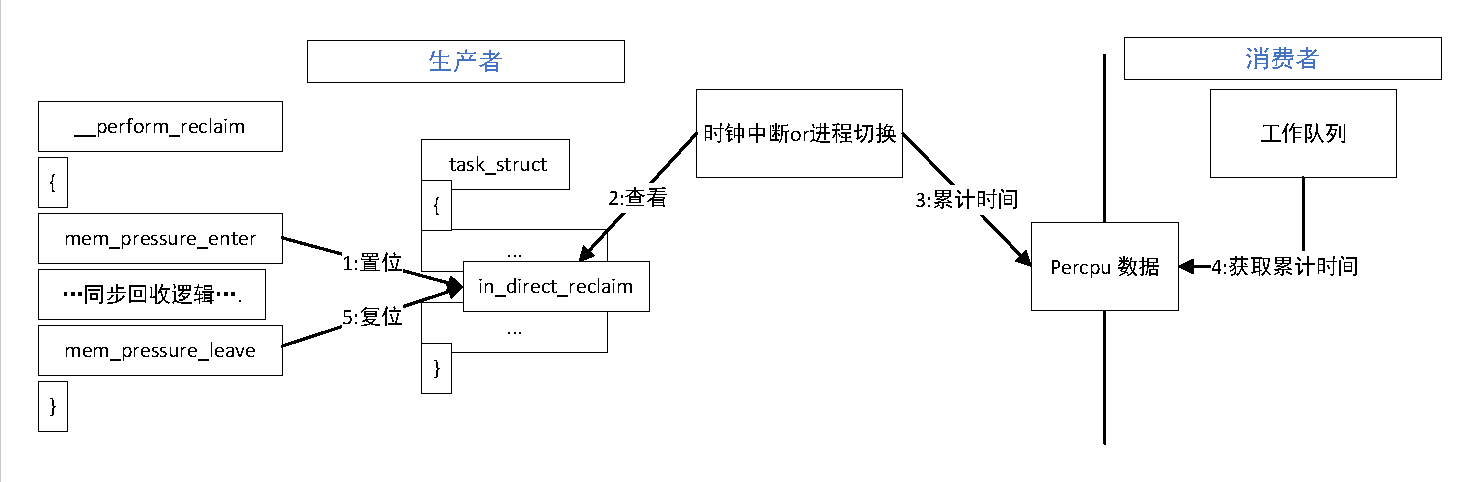
\includegraphics[width=\textwidth,keepaspectratio]{生产者和消费者.pdf}
    \caption{生产者消费者架构图}
    \label{fig:producer-consumer}
\end{figure}

系统实现如\ref{fig:producer-consumer}, 采用生产者消费者模式构建内存压力实时监控与评估框架。该模式通过解耦数据采集与数据处理两个核心功能模块。生产者模块负责采集内存回收过程中的时间片数据,而消费者模块则周期性地处理这些数据,计算内存压力指标。两者共享Per-CPU数据,它统计了每个CPU中发生内存同步回收的时间。具体的信息详见\ref{tab:sensor_data}。同时本文在 Linux 中 task\_struct 中 in\_mem\_mempressure 表示这个进程在处理同步内存回收了。

\begin{table}[htbp]
    \centering
    \caption{Per-CPU 变量}
    \label{tab:sensor_data}
    \begin{tabular}{ccc}
        \toprule
        成员名称& 数据类型     & 描述                                        \\ \midrule
        in\_direct\_reclaim & bool & 当前CPU是否处于同步内存回收状态\\
        \midrule
        time & u32 & 上一次累积时间的时间戳\\
        \midrule
        total\_time &u32&当前CPU处于同步内存回收状态的累积时间\\
        \midrule
        total\_time\_prev&u32&上一次统计时CPU处于同步内存回收状态的累积时间\\
        \midrule
        total\_work\_time&u32&当前CPU处于工作状态的累积时间\\
        \midrule
        total\_work\_time\_prev&u32&上一次统计时CPU处于工作状态的累积时间\\
        \bottomrule
    \end{tabular}
  \end{table}

生产者模块的核心功能是精确捕获内核中与内存回收相关的状态切换时间信息。为实现这一目标,生产者在同步内存回收的起始和结束时刻改变状态。具体而言,当系统发生直接内存回收时,即进程在分配内存时因内存不足而触发同步回收操作,生产者立即改变状态。当同步回收过程结束,进程恢复正常执行时,生产者再次改变状态,并计算累积时间。同时每次时钟中断的时候,它会进行累积时间。除此之外,生产者需要和调度系统交互,用来控制时钟中断收集间隔,因为当这个线程调度出去的时候,CPU就不会花费时间来处理同步内存回收,当调度进来的时候,生产者就需要重新计算,所以需要和调度系统交互并且在task\_struct中in\_mem\_mempressure标志来表示这个线程是否在处理同步内存回收。

消费者模块使用工作队列来实现,周期的从Per-CPU中读取读取,进行聚合,在\ref{sec:工作队列}介绍了选用工作队列的原因,在\ref{sec:内存压力计算算法}中介绍了详细的算法实现。


\subsection{生产者工作流程}

\begin{figure}[htbp]
    \centering
    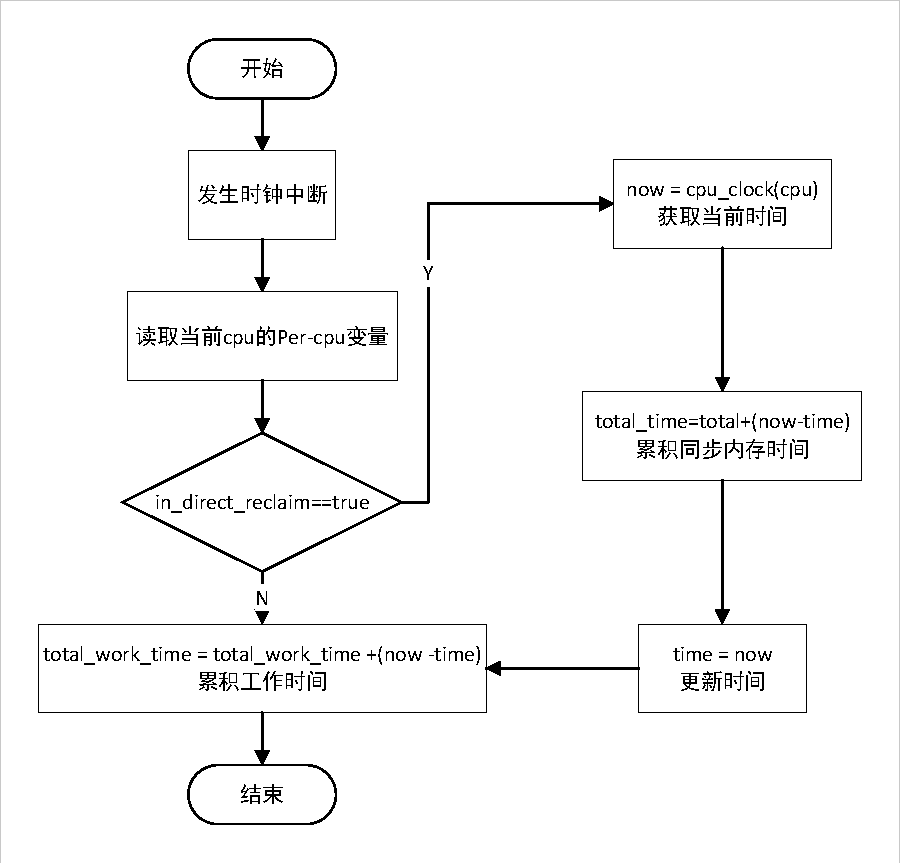
\includegraphics[width=0.8\textwidth,keepaspectratio]{时钟中断.pdf}
    \caption{时钟中断流程图}
    \label{fig:time-ticker}
\end{figure}
图\ref{fig:time-ticker} 所示为时钟中断处理流程。该流程始于时钟中断的触发,随后系统读取当前CPU的Per-CPU变量,并进入一个关键判定节点:判断in\_direct\_reclaim标志的状态。

若in\_direct\_reclaim为真,表明当前CPU正处于直接内存回收状态。此时,系统会执行以下操作:首先,通过cpu\_clock(cpu)函数获取当前时间戳,记为now;其次,计算时间差(now - time),并将其累加到total\_time变量中,用于统计同步内存回收所消耗的时间;最后,将now的值赋给time,以更新当前时间记录。这一过程确保了系统能够准确记录CPU在同步内存回收上花费的时间。

若in\_direct\_reclaim为假,则表明当前CPU未处于直接内存回收状态。此时,系统会计算时间差(now - time),并将其累加到total\_work\_time变量中,用于统计CPU在工作状态下的时间消耗。无论in\_direct\_reclaim的真假,流程最终都会汇聚至结束节点,完成一次时钟中断的处理。


此外,在进程切换时,系统会检查task\_struct中的in\_mem\_mempressure标志。如果当前进程的in\_mem\_mempressure为true,则表明该进程涉及内存压力,此时需要修改Per-CPU变量中的in\_direct\_reclaim标志,以表示当前CPU不再花费时间进行同步内存回收。反之,如果要切换进来的进程的in\_mem\_mempressure为true,则需要将Per-CPU变量中的in\_direct\_reclaim标志设置为true,表示当前CPU需要花费时间进行同步内存回收。

\subsection{消费者实现与并发安全保障}
\label{sec:consumer_implementation}

\subsubsection{基于工作队列的消费者实现}
\label{sec:工作队列}
在内存压力监控系统的消费者模块实现中,本文选择采用Linux内核工作队列机制,主要基于以下三方面考量:
\begin{enumerate}
    \item 内存压力计算过程涉及锁获取和较长时间的数据处理,必须在进程上下文中执行。工作队列提供的进程上下文执行环境,能够安全地处理可能引起睡眠的操作,这是中断上下文所不允许的。
    \item 压力监测需要周期性执行,工作队列的延迟执行机制(queue\_delayed\_work)不仅提供了高效的定时功能,还实现了完善的周期补偿。即使在系统负载较高导致某些执行周期被延迟时,工作队列能够通过公式(\ref{eq:missed_periods})计算错过的周期数并进行补偿,确保监测的连续性和数据的一致性。
    \item 工作队列的自适应特性使其能根据系统负载动态调整执行频率,在保证监测效果的同时最小化性能开销。相比于自行实现专用内核线程,工作队列机制显著降低了边界条件处理的复杂度,避免了诸如线程创建、销毁和唤醒等底层细节的处理。
\end{enumerate}

本文的实现使用以下工作队列API完成内存压力监测的周期性执行:

\begin{table}[htbp]
\centering
\caption{内存压力监测系统使用的工作队列API}
\label{tab:workqueue_api}
\begin{tabular}{cc}
\toprule
\textbf{API} & \textbf{在内存压力监测中的应用} \\
\midrule
alloc\_workqueue & 创建专用内存压力监测工作队列 \\
INIT\_DELAYED\_WORK & 初始化周期性监测任务 \\
queue\_delayed\_work & 按指定周期调度监测任务 \\
\bottomrule
\end{tabular}
\end{table}

具体而言,消费者模块通过工作队列周期性地调用算法\ref{alg:mem_pressure_optimized},依次执行多核加权聚合、时间戳更新和指数平滑计算,完成内存压力的实时评估。该实现不仅确保了监测过程的稳定性和可靠性,还使监测代码能够与工作负载高效共存,最小化了系统性能影响。

\subsubsection{临界区的保护}

在生产者消费者模型中,生产者负责采集内存回收过程中的累积时间,而消费者(工作队列)则负责处理这些数据,计算并输出内存压力指标。为了确保数据在并发环境下的完整性和一致性,同时兼顾性能,需要对临界区进行精细的保护。

在详细阐述临界区保护策略之前,有必要先介绍本研究所采用的核心同步机制:序列锁(Seqlock)。序列锁是 Linux 内核提供的一种轻量级同步原语,特别适用于读多写少且写操作简短的场景。其基本原理如图 \ref{fig:seqlock} 所示。序列锁维护一个序列计数器,写操作通过递增该计数器来标识数据更新的开始和结束(奇数表示写操作进行中,偶数表示无写操作)。读操作在开始时记录序列号 read\_seqbegin(),并在读取完成后再次检查序列号 read\_seqretry()。如果序列号发生变化,则表明在读取过程中发生了写操作,读操作需要重试,以确保读取到一致的数据。

\begin{figure}[H]
    \centering
    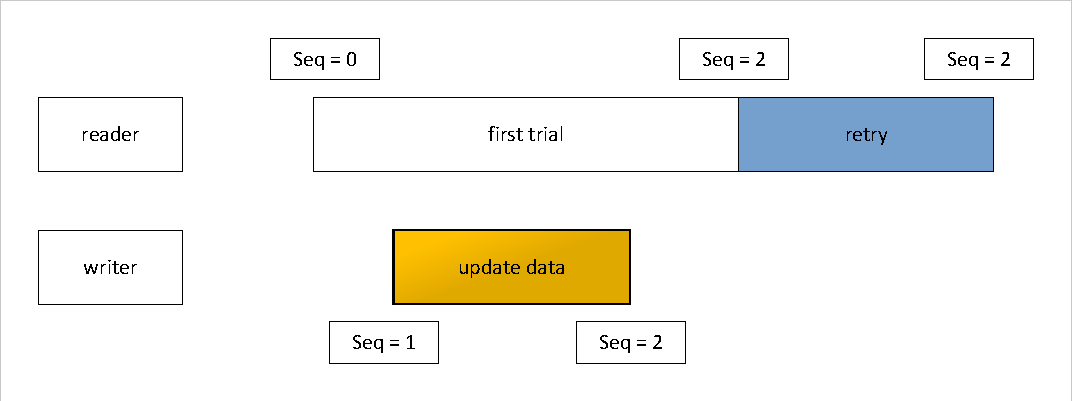
\includegraphics[width=\textwidth,keepaspectratio]{seqlock.pdf}
    \caption{序列锁(Seqlock)原理示意图}
    \label{fig:seqlock}
\end{figure}

在本研究中,需要重点保护的临界区主要包括以下三类:

\begin{enumerate}
    \item  Per-CPU 数据:每个 CPU 核心维护一份独立的数据结构,在表\ref{tab:sensor_data}中可以看到存储了CPU的统计信息。尽管 Per-CPU 变量在更新时本身具有原子性,无需额外加锁,但考虑到消费者需要读取所有 CPU 的 Per-CPU 数据进行聚合计算,因此仍需采取适当的同步措施。
    \item 全局统计信息:一个全局静态变量,用于存储所有 CPU 停顿时间的累加值,以及用于平滑计算的历史统计数据。该变量的访问涉及多个 CPU 的数据聚合,因此需要严格的保护。
    \item task\_struct->in\_mem\_mempressure 标志:task\_struct 中的一个标志位,用于标识当前进程是否涉及内存压力。该标志用于指导每次进程切换时,是否需要更新Per-CPU中的in\_direct\_reclaim标志。
\end{enumerate}

基于对这些数据结构特点和访问模式的深入分析,本研究采用了三种具有针对性的临界区保护策略,以平衡数据一致性与系统性能。

对于Per-CPU数据中的累计时间,系统选择了序列锁保护机制。这一选择主要基于以下考量:首先,时钟中断处理函数需要频繁更新该数据,而中断处理程序不能被阻塞,序列锁恰好提供了无阻塞写入能力;其次,Per-CPU数据结构相对简单,多为32位或64位无符号整型,写操作(累加时间)执行快速,读取时可整体复制,这些特性与序列锁的适用条件高度吻合;此外,内存同步回收通常不是高频事件,对停顿时间的累加操作较少,构成典型的读多写少场景,这与序列锁的设计理念完全契合。

\begin{algorithm}[htbp]
    \caption{Memory Pressure Calculation}
    \label{alg:mem_pressure_optimized}
    \SetAlgoLined
    \DontPrintSemicolon

    \Input{
            \(\text{total\_time}_i, \text{total\_time\_prev}_i, \text{total\_work\_time}_i, \text{total\_work\_time\_prev}_i\) (for each CPU \(i\));
            \(\text{mem\_pressure\_time}, \text{mem\_pressure\_time\_prev}\),
            \(\text{mem\_pressure\_prev}, \text{next\_update\_time}, \text{last\_update\_time}, T, \text{exp}\);
    }
    \Output{updated 
         \(\text{mem\_pressure\_prev}, \text{mem\_pressure\_time\_prev},\)
         \(\text{next\_update\_time}, \text{last\_update\_time}\)}

    \BlankLine

    \(\text{weight\_pressure\_time}, \text{work\_time} \gets \text{calculate\_weighted\_pressure\_time}(\text{cpu\_data})\)\;
    \(\text{mem\_pressure\_time} \gets \lfloor \text{weight\_pressure\_time}/\max(\text{work\_time},1)\rfloor\)\;

    \(\text{next\_update\_time}, \text{last\_update\_time}, \text{missed}, \text{period} \gets\) \(\text{update\_timestamps}(\text{sched\_clock}(), \text{next\_update\_time}, \text{last\_update\_time}, T)\)\;

    \(\text{mem\_pressure\_prev} \gets \text{exponential\_smoothing}(\)
    \qquad \(\text{mem\_pressure\_time}, \text{mem\_pressure\_time\_prev},\)
    \qquad \(\text{period}, \text{mem\_pressure\_prev}, \text{exp}, \text{missed})\)\;
\end{algorithm}
而对于全局统计信息,考虑到其操作复杂性和访问特点,本研究采用了互斥锁(Mutex)保护机制。互斥锁提供了更强的互斥性,适合保护涉及较长计算时间或复杂数据结构的操作。全局统计信息的更新需要聚合多个CPU的数据并进行历史数据的平滑计算,这些操作相对耗时且复杂。尽管互斥锁可能引入一定的性能开销,但由于全局统计信息的访问频率相对较低,通常只在消费者周期性执行时进行,因此这种开销在实际应用中处于可接受范围内。
\begin{algorithm}[H]
    \caption{calculate\_weighted\_pressure\_time}
    \label{alg:calculate_weighted_pressure_time}
    \SetAlgoLined
    \DontPrintSemicolon
    \Input{\(\text{total\_time}_i, \text{total\_time\_prev}_i, \text{total\_work\_time}_i, \text{total\_work\_time\_prev}_i\) (for each CPU \(i\))}
    \Output{\(\text{weight\_pressure\_time}, \text{work\_time}\)}
    \(\text{weight\_pressure\_time} \gets 0,\quad \text{work\_time} \gets 0\)\;
    \For{each CPU \(i\)}{
        \(\text{weight\_pressure\_time} \gets \text{weight\_pressure\_time} + (\text{total\_time}_i - \text{total\_time\_prev}_i) \times (\text{total\_work\_time}_i - \text{total\_work\_time\_prev}_i)\)\;
        \(\text{work\_time} \gets \text{work\_time} + (\text{total\_work\_time}_i - \text{total\_work\_time\_prev}_i)\)\;
    }
    \Return{\(\text{weight\_pressure\_time}, \text{work\_time}\)}
    \end{algorithm}
至于task\_struct中的in\_mem\_mempressure标志,系统采用了一种巧妙的隐式保护策略。该标志在同步内存回收开始时置位,结束时复位,这些操作通常发生在进程调度环境中。由于内核在操作过程中已持有相应CPU的运行队列锁并关闭本地中断,这自然形成了一道保护屏障,防止其它CPU或中断对当前进程的调度产生干扰。因此,在时钟中断处理函数中检查该标志时,运行队列锁的存在保证了当前进程不会被调度到其它CPU,使得直接访问该标志是安全的,无需引入额外的锁机制。这种复用已有同步原语的策略,不仅简化了系统设计,还有效降低了同步开销。

\begin{algorithm}[H]
    \caption{update\_timestamps}
    \label{alg:update_timestamps}
    \SetAlgoLined
    \DontPrintSemicolon
    \Input{\(\text{now}, \text{next\_update\_time}, \text{last\_update\_time}, T\)}
    \Output{ \(\text{next\_update\_time}, \text{last\_update\_time}, \text{missed}, \text{period}\)}
    \If{\(\text{now} < \text{next\_update\_time}\)}{
    \Return{\(\text{next\_update\_time}, \text{last\_update\_time}, 0, 0\)}
    }
    \(\text{missed} \gets \lfloor(\text{now}-\text{next\_update\_time})/T\rfloor\)\;
    \(\text{next\_update\_time} \gets \text{next\_update\_time} + (\text{missed}+1) \times T\)\;
    \(\text{period}\gets \text{now}-\text{last\_update\_time}\)\;
     \(\text{last\_update\_time}\gets \text{now}\)\;
    \Return{\(\text{next\_update\_time}, \text{last\_update\_time}, \text{missed}, \text{period}\)}
    \end{algorithm}
总体而言,通过这三种针对性的临界区保护策略,本框架在确保数据一致性和完整性的前提下,最大限度地降低了同步开销,从而显著提升了系统的整体性能和响应能力。实验结果表明,这种差异化的保护策略在实际应用中表现出色,能够有效地平衡保护强度与性能开销之间的权衡。

\subsection{内存压力计算工程实现}
\label{sec:内存压力计算算法}
本节聚焦于内存压力量化算法的工程实现。基于\ref{sec:基于同步内存回收延迟的内存压力量化算法}的理论模型,本文设计了一套高效的算法体系,实现了从原始数据采集到最终压力指标输出的完整计算流程。核心实现遵循先聚合、再校准、后平滑的处理逻辑,同时采用定点数运算优化性能。



 \begin{algorithm}[H]
     \caption{exponential\_smoothing}
     \label{alg:exponential_smoothing}
     \SetAlgoLined
     \DontPrintSemicolon
     \Input{
         \begin{varwidth}{\linewidth}
           \(\text{mem\_pressure\_time}, \text{mem\_pressure\_time\_prev}, \text{period}\)\\
           \(\text{mem\_pressure\_prev}, \text{exp}, \text{missed}\)
         \end{varwidth}
     }
     \Output{\(\text{mem\_pressure\_prev}\)}
     
     \(\text{sample\_time}\gets \text{mem\_pressure\_time}-\text{mem\_pressure\_time\_prev}\)\;
     \If{\(\text{sample\_time}>\text{period}\)}{
         \(\text{sample\_time}\gets \text{period}\)
     }
     \(\text{mem\_pressure\_time\_prev} \gets \text{mem\_pressure\_time\_prev} + \text{sample\_time}\)\;
     \(\text{tmp\_mem\_pressure}\gets \lfloor(\text{sample\_time}\times 100\times 2^{10})/\text{period}\rfloor\)\;
     \If{\(\text{missed}>0\)}{
       \(\text{exp} \gets \text{fixed\_power\_int}(\text{exp}, \text{missed})\)
     }
     \(\text{new\_mem\_pressure}\gets \text{mem\_pressure\_prev}\times \text{exp} + \text{tmp\_mem\_pressure}\times(2^{10}-\text{exp})\)\;
     \If{\(\text{mem\_pressure\_prev}>\text{tmp\_mem\_pressure}\)}{
       \(\text{new\_mem\_pressure} \gets \text{new\_mem\_pressure} + (2^{10}-1)\)
     }
     \(\text{mem\_pressure\_prev}\gets \lfloor \text{new\_mem\_pressure}/2^{10}\rfloor\)\;
     \Return{\(\text{mem\_pressure\_prev}\)}
 \end{algorithm}
算法\ref{alg:mem_pressure_optimized}展示了内存压力计算的主流程。第1行调用\\
 calculate\_weighted\_pressure\_time 函数实现\ref{sec:weighted_aggregation}节提出的多核加权聚合模型。第2行将加权后的内存压力时间转换为百分比表示,同时通过max函数处理工作时间为零的边缘情况。第3行调用 update\_timestamps 函数实现时间校准机制,处理采样周期偏移问题。第4行应用 exponential\_smoothing 函数实现指数平滑处理,输出最终压力值。

算法\ref{alg:calculate_weighted_pressure_time}实现了多核加权聚合。第3行是该算法的核心,它通过回收时间增量与工作时间增量的乘积累加,实现了公式\ref{eq:weighted_aggregation}中的权重聚合,避免了空闲核心的稀释效应。这种实现方式优于显式维护权重数组的方法,具有更高的计算效率。第4行累加工作时间增量,为后续计算压力百分比提供分母。

算法\ref{alg:update_timestamps}处理采样时间管理。第1-2行检查是否达到下次更新时间,避免过早执行。第3行根据公式\ref{eq:missed_periods}计算错过的周期数。第4行应用公式\ref{eq:next_execution}更新下次执行时刻,保持采样相位一致性,防止时间偏移累积。这种相位校准机制确保了即使在系统负载波动时,内存压力监测依然能保持连续稳定的采样节奏。
算法\ref{alg:exponential_smoothing}实现了指数平滑处理。第1-2行计算并限制样本时间,应用\ref{sec:time_calibration_and_data_processing}节提出的截断补偿机制。第4行将样本时间转换为百分比并用定点数表示,实现\ref{sec:fixed_point_optimization}节的定点数优化。第5-6行处理连续多个周期未更新的情况,使用fixed\_power\_int函数实现指数加速收敛。第7行使用指数加权公式计算新的内存压力值,定点数表示的exp和$(2^{10}-\text{exp})$分别对应公式\ref{eq:EMA}中的\(\alpha\)和\((1-\alpha)\)。第8-9行是工程优化,在压力下降时进行微调,提高系统对压力缓解的响应性。
\SetKwFunction{FixedPowerInt}{fixed\_power\_int}
\SetKwProg{Fn}{Function}{:}{}
算法\ref{alg:helper_functions}实现了定点数快速幂计算。第2行初始化结果为定点数的1.0。第3-11行实现二进制快速幂算法,时间复杂度为$O(\log n)$。第6行和第9行中的$(expr + 2^9) \gg 10$操作实现了定点数乘法中的四舍五入,确保计算精度。

\begin{algorithm}[htb]
    \caption{fixed\_power\_int}
    \label{alg:helper_functions}
    \SetKwFunction{FixedPowerInt}{fixed\_power\_int}
    \SetKwProg{Fn}{Function}{:}{}

    \Fn{\FixedPowerInt(\(x\), \(n\))}{
        \(result \gets 2^{10}\) \;
        \If{\(n > 0\)}{
            \While{true}{
                \If{\((n \land 1) \neq 0\)}{
                    \(result \gets (result \times x + 2^9) \gg 10\)\;
                }
                \(n \gets n \gg 1\)\;
                \If{\(n = 0\)}{\textbf{break}}
                \(x \gets (x \times x + 2^9) \gg 10\)\;
            }
        }
        \Return \(result\)\;
    }
\end{algorithm}



\section{本章小结}
本章详细阐述了基于同步内存回收延迟的内存压力量化算法的设计与实现。首先,通过分析同步回收延迟与内存压力的关联性,提出了基于同步回收延迟的内存压力量化模型,并建立了相应的数学表征。其次,针对多核系统中的负载不均衡问题,设计了多核加权聚合算法,有效降低了空闲核心对压力评估的干扰。此外,引入指数移动平均算法对压力数据进行平滑处理,减少了短期波动的影响,同时采用定点数优化技术显著提升了计算效率。在实现层面,基于生产者消费者模式构建了内存压力实时监控框架,通过序列锁和互斥锁等同步机制确保了数据的一致性和完整性。最后,详细介绍了内存压力计算算法的具体实现,包括加权压力时间计算、时间戳更新以及指数平滑更新等核心模块。